\documentclass[12pt]{article}

% Import packages
\usepackage[margin=1in]{geometry}
\usepackage{enumitem}
\usepackage[utf8]{inputenc}
\usepackage[english]{babel}
\usepackage{amsthm}
\usepackage{amsmath}
\usepackage{mathtools}
\usepackage{amssymb}
\usepackage{algorithmicx}
\usepackage[ruled,vlined]{algorithm2e}
\usepackage{commath}
\usepackage{float}
\usepackage{mathrsfs}
\usepackage{bm}
\usepackage{bbm}
\usepackage{tikz}
\usetikzlibrary{decorations.pathreplacing}
\usepackage[colorlinks=true,linkcolor=blue]{hyperref}
\usepackage{bookmark}
\usepackage{titlesec}
\setcounter{secnumdepth}{4}
\usepackage{tcolorbox}
\tcbuselibrary{breakable}
\allowdisplaybreaks

% Theorems and Lemmas
\newtheorem{thm}{Theorem}
\newtheorem{lem}{Lemma}
\newtheorem{axiom}{Axiom}
\newtheorem{corollary}{Corollary}

\theoremstyle{definition}
\newtheorem{example}{Example}[section]
\newtheorem{definition}{Definition}
\newtheorem{remark}{Remark}

% Macros
\newcommand{\pr}[1]{\mathbb{P}\del{#1}}

\newcommand{\E}[1]{\mathbb{E}\sbr{#1}}

\newcommand{\var}[1]{\mathrm{Var}\del{#1}}

\newcommand{\fl}[1]{\mathrm{fl}\del{#1}}

\newcommand{\pb}{\boxed{+}\,}

\begin{document}
\begin{titlepage}
\title{Programming Solutions}
\author{Lu Vy}
\date{September 28, 2020}
\maketitle
\thispagestyle{empty}
\end{titlepage}

\section{Summary}
We compare three addition algorithms and demonstrate their theoretical error bounds. Using various sums, we verify that these sums are correct, and that they are stable, as assured by the mathematics. We also verify that addition is a well conditioned problem.

\section{Problem Statement}
We numerically verify (1) the conditioning upper bound on addition problems, and (2) the stability of three addition algorithms. The three algorithms in question are the recursive cumulative sum in single precision IEEE arithmetic, the binary fan-in tree, and the cumulative sum again in double precision (algorithms 1, 2, and 3 hereafter).  Before the stability analysis, we show that the three algorithms produce correct results (as correct as they can be, given their limitations). The shortcomings of $\mathcal{F}\del{\beta,t,L,U}$ relative to $\mathbb{R}$ are reproduced analogously using the shortcomings of single precision floats relative to double precision floats.

\section{Mathematics}
We pose the problem in the following way: find $x \in \mathbb{R}$ that satisfies $$F\del{x,\bf{d}} = \del{d_1 + d_2 + \cdots + d_n} - x = 0$$ given fixed $\mathbf{d} = \del{d_1,\dots,d_n}^T \in \mathbb{R}^n$ \cite{quateroni}. Under the constraint $F\del{x,\bf{d}} = 0$, we may view $x$ as a function of $\mathbf{d}$. This $x\del{\mathbf{d}}$ is well conditioned because
\begin{align*}
\abs{\frac{x\del{\mathbf{d+\Delta d}}-x\del{\mathbf{d}}}{x\del{\mathbf{d}}}} &=
\abs{\frac{\sum_i \del{d_i + \Delta d_i}-\sum_i\del{d_i}}{\sum_i\del{d_i}}} = \abs{\frac{\sum_i \Delta d_i}{\sum_i d_i}} \\ &\leq \frac{\sum_i \abs{\Delta d_i}}{\abs{\sum_i d_i}} = \frac{\sum_i\abs{d_i}}{\abs{\sum_i d_i}}\frac{\sum_i \abs{\Delta d_i}}{\sum_i \abs{d_i}} 
= \kappa_r\frac{\norm{\mathbf{\Delta d}}_1}{\norm{\mathbf{d}}_1}.
\end{align*}
One may bound the absolute error $\abs{x\del{\mathbf{d+\Delta d}}-x\del{\mathbf{d}}} < \kappa_a \norm{\mathbf{\Delta d}}_1$ in a similar way \cite{lec3}. Here, $\kappa_r = \frac{\sum_i\abs{d_i}}{\abs{\sum_i d_i}}$ and $\kappa_a = \sum_i\abs{d_i}$ denote the relative and absolute \textit{condition numbers}.


The three algorithms merely approximate $x\del{\mathbf{d}}$. In this investigation, we consider two sources of error that prevent us from attaining $x\del{\mathbf{d}}$ exactly \cite{lec2}:
\begin{enumerate}
\item finite precision representation of real numbers. These not only perturb the data $d_1,\dots,d_n$, but also restrict the range of values that $x$ may take.
\item accumulation of errors due to floating point arithmetic.
\end{enumerate}
If $\hat{x}$ is an approximation of $x$, then two quantities of interest are $\abs{\hat{x} - x}$ and $\abs{\frac{\hat{x}-x}{x}}$. We call the former \textit{absolute forward error} and the latter \textit{relative forward error}. We derive upper bounds for each.

In fact, we show that all three algorithms are backwards stable. That is, the errors are no greater than
\begin{align*}
\abs{\hat{x}-x} \leq \kappa_a p\del{n} u \qquad \text{and} \qquad
\abs{\frac{\hat{x}-x}{x}} \leq \kappa_r p\del{n} u,
\end{align*}
for some $p\del{n}$, and for each approximate solution $\hat{x}$, there exists a vector $\Delta \mathbf{d}$ (small relative to $\mathbf{d}$) that satisfies $F\del{\hat{x},\mathbf{d}+\Delta\mathbf{d}}=0.$ Here, $u = 2^{-24}$ denotes \textit{unit round off}.

\subsection{Algorithm 1}
It has been shown \cite{lec3} that if $\mathbf{\xi} = \del{\xi_1,\dots,\xi_n}^T$ is a vector of floating point numbers, then the errors have the approximate bounds
\begin{align*}
\abs{\hat{x}_1\del{\xi}-x\del{\xi}} &\lesssim  \kappa_a n u\\
\abs{\frac{\hat{x}_1\del{\xi}-x\del{\xi}}{x\del{\xi}}} &\lesssim  \kappa_r n u.
\end{align*}
If instead we require the data $\mathbf{d} = \del{d_1,\dots,d_n}^T$ to be real valued, then this does not change the bounds (provided that they are within range, i.e. not too large). Indeed for each $d \in \mathbb{R}$ (within range), there exists $\xi \in \mathcal{F}\del{\beta,t,L,U}$ and $\delta \in \del{-u,u}$ for which $d = \xi\del{1 + \delta}$. Thus substitution of $\mathbf{d}$ into $\mathbf{\xi}$ does not change the order of $p\del{n} \in \mathcal{O}\del{n}$. 

To show that $\hat{x}_1\del{\mathbf{d}}$ is backwards stable, recall \cite{lec4} that we may express $\hat{x}_1\del{\mathbf{d}}$ in the form
$$
\hat{x}_1\del{\mathbf{d}} = \sum_{i=1}^n d_i\del{1 + \eta_i},
$$
where $\abs{\eta_i} \lesssim nu$. Hence, $\hat{x}_1\del{\mathbf{d}}$ actually solves the problem with data $$\mathbf{d + \Delta d}=\del{d_1\del{1 + \eta_1},  \dots, d_n\del{1 + \eta_n}}^T.$$ Our backward error (using the $L_1$ norm) is
$$
\norm{\Delta \mathbf{d}}_1 = \norm{\del{d_1\eta_1, \dots, d_n\eta_n}^T}_1 = \sum_{i=1}^n\abs{d_i \eta_i} \leq \norm{\mathbf{d}}_1 \norm{\mathbf{\eta}}_1
$$
which is small relative to $\norm{\mathbf{d}}_1$ because each $\eta_i$ is small.

\subsection{Algorithm 2}
Assume that $n = 2^k$ for some $k \in \mathbb{N}$. If this is not the case, then take $\tilde{n} = 2^{\lceil{\log_2 n}\rceil}$ and let $d_{n+1} = \cdots = d_{\tilde{n}} = 0$. For floating point $\xi$, we claim that
\begin{align*}
\abs{\hat{x}_2\del{\xi} - x\del{\xi}} &\lesssim \kappa_a \del{\log_2 n}u \\
\abs{\frac{\hat{x}_2\del{\xi} - x\del{\xi}}{x\del{\xi}}}  &\lesssim \kappa_r\del{\log_2 n}u.
\end{align*}
That is, $p\del{n} \in \mathcal{O}\del{\log_2 n}$ for the binary fan-in tree. For proof, see 1.3.c in the written homework solutions. As was the case before, real valued data does not change the order of $p\del{n}$; we may take $p\del{n} = 1 + \log_2 n$ if we wish to be conservative.



Just like algorithm 1, $\hat{x}_2\del{\mathbf{d}}$ solves the problem with data $\del{d_1\del{1+\eta_1},\dots,d_n\del{1+\eta_n}}^T$. We attain a similar expression for the backwards error (see homework problem 1.3.b.), with the $\eta_i$ being different, but still small ($\abs{\eta_1} \lesssim \del{1+\log_2 n}u$).

\subsection{Algorithm 3}
Unit round off for double precision floats $u_{dp} = 2^{-53}$ is $2^{29}$ times smaller than that of single precision $u_{sp} = 2^{-24}$. We therefore neglect the accumulation of rounding error due to double precision addition. This may be problematic when $n \gg 2^{29}$, but we do not consider such sums here here. The algorithm in question is
\begin{align*}
\sigma_{1:n} &= \fl{\fl{d_1} + \fl{d_2} +  \cdots  + \fl{d_n}} \\
&= \fl{d_1\del{1 + \delta_1} + d_2\del{1 + \delta_2} + \cdots + d_n\del{1 + \delta_n}} \\
&= \del{d_1\del{1 + \delta_1} + d_2\del{1 + \delta_2} + \cdots + d_n\del{1 + \delta_n}}\del{1 + \delta_{n+1}} \\
&= \sum_{i=1}^n d_i \del{1 + \delta_i}\del{1 + \delta_{n+1}} \\
&= \sum_{i=1}^n d_i \del{1 + \eta_i},
\end{align*}
where
$$
\del{1 + \eta_i} = \del{1 + \delta_i}\del{1 + \delta_{n+1}} \implies \abs{\eta_i} \lesssim 2u.
$$
It follows that
\begin{align*}
\abs{\hat{x}_2 - x} &\lesssim \sum_{i=1}^n\abs{d_i}2u  = 2\kappa_a u \\
\abs{\frac{\hat{x}_2 - x}{x}}  &\lesssim \frac{\sum_{i=1}^n\abs{d_i}}{\abs{\sum_{i=1}^n d_i}}2u = 2\kappa_r u.
\end{align*}
In particular, $p\del{n} \in \mathcal{O}\del{1}$.

As before, $\hat{x}_3\del{\mathbf{d}}$ solves the problem with data $\mathbf{d}=\del{d_1\del{1+\eta_1},\dots,d_n\del{1+\eta_n}}^T$, and the backward error is small: $\abs{\eta_i} \lesssim 2u$.

\section{Algorithm and Implementation}
Each algorithm takes in an array of length $n$ and adds the first $k \leq n$ terms.

It is straightforward to program algorithm 1. All that is needed is an accumulator and a for-loop. By float, that is meant single precision floating point digit. For algorithm 2, we add in pairs until we reduce the array to a single number, which is the value returned. If there is an odd term, it is added to 0. Algorithm 3 is the same as algorithm 1, except the accumulator is double precision, and every float added to it must also first be converted to double precision.

For the purposes of analysis, we need an algorithm that takes in double precision floats and outputs a double precision float. This is to represent the ``exact'' sum when one is not known in closed form. Because $u_{dp} \ll u_{sp}$, it does not matter which form of addition we use, but we opt for the binary fan-in tree because its error is $\mathcal{O}\del{\log_n n u_{dp}}$.

\begin{algorithm}[H]
\SetAlgoLined
\KwData{array of single precision floats $\xi_1,\dots,\xi_n$, integer $k \leq n$ of terms to be added}
\KwResult{single precision float $S$}
initialization\;
float $S \leftarrow 0$\;
 \For{$i=1$ \KwTo $k$}{
 	$S \leftarrow S + \xi_i$\;
 }
 \Return{$S$}\;
 \caption{Single precision accumulation}
 \label{algorithm1}
\end{algorithm}

\begin{algorithm}[H]
\SetAlgoLined
\KwData{array of single precision floats $\xi_1,\dots,\xi_n$, integer $k \leq n$ of terms to be added}
\KwResult{single precision float $S$}
initialization\;
duplicate array $\mathbf{v} \leftarrow \sbr{\xi_n,\dots,\xi_n}$\;
\While{$k > 1$}{
\For{$i=0$ \KwTo $\lfloor{\frac{k}{2}\rfloor}$}{
		$\mathbf{v} \leftarrow \mathbf{v}\sbr{2i} + \mathbf{v}\sbr{2i+1}$\;
	}
\eIf{$k$ is even}{$k \leftarrow \frac{k}{2}$\;}{$k \leftarrow \lceil{\frac{k}{2}\rceil}$\;}
}
 \Return{$\mathbf{v}\sbr{0}$}\;
 \caption{Binary fan-in tree}
\end{algorithm}

\begin{algorithm}[H]
\SetAlgoLined
\KwData{array of single precision floats $\xi_1,\dots,\xi_n$, integer $k \leq n$ of terms to be added}
\KwResult{single precision float $S$}
initialization\;
double $S \leftarrow 0$\;
 \For{$i=1$ \KwTo $k$}{
 	double $d \leftarrow \xi_i$\;
 	$S \leftarrow S + d$\;
 }
 float $out \leftarrow S$\;
 \Return{$out$}\;
 \caption{Double precision accumulation}
\end{algorithm}

\section{Experimental Design and Results}
The three tasks at hand are: correctness, conditioning, and stability. We conduct two tests for each, for a total of six.
\subsection{Correctness}
Are the three algorithms accurate? To answer this, we consider Taylor series. Taylor's remainder theorem gives us a theoretical upper bound on their convergence rates: for each $f$ with at least $n$ derivatives in a neighborhood of $0$, we have that
$$
f\del{x} = f\del{0} + f'\del{0}x + \cdots + \frac{f^{\del{n-1}}\del{0}}{\del{n-1}!}x^{n-1} + \frac{f^{\del{n}}\del{c}}{n!}x^{n}
$$
for some $c \in \del{0,x}$ \cite{kincaid}. Thus error of the $\del{n-1}^{th}$ term sum is of the order $\mathcal{O}\del{\frac{1}{n!}}$.
\subsubsection{Test 1}
Consider the series $\sum_{k=0}^\infty \frac{1}{k!} \to e$. We consider the first $15$ terms, for anything after $k = 10$ is less than round off error: $\frac{1}{10!} > u > \frac{1}{11!}$. The mathematics suggests that
$$
\mathrm{err}_n = \abs{e - \sum_{k=0}^{n-1} \frac{1}{k!}} = \frac{e^c}{n!} \leq \frac{e}{n!}, \qquad c \in \del{0,1}.
$$
An upper bound for the relative error is therefore $\mathrm{err}_{\text{rel}} \leq \frac{1}{n!}$. Our experiment will verify whether this upper bound holds for $n \in \cbr{2,\dots,15}$. In accordance with lecture notes 4 \cite{lec4}, the cumulative sums will go from smallest to largest.

\subsubsection{Test 2}
Consider the series $\sum_{k=0}^\infty\frac{\del{-1}^k}{\del{2k+1}!} \to \sin\del{1}$. We consider the first $10$ terms, for the same reason specified in test 1. The mathematics suggests that
$$
\mathrm{err}_n = \abs{\sin\del{1}-\sum_{k=0}^{n-1}\frac{\del{-1}^k}{\del{2k+1}!}} = \frac{\sin\del{c}}{2n!} \leq \frac{1}{2n!}.
$$

\subsection{Conditioning}
How much will perturbations in the data affect the solution? The mathematics says that summation is a well conditioned problem, so any change in the data should result in a proportionate change in the solution. To verify this, we generate fix $n$ and generate a noise vector $\mathbf{\Delta d}$ with IID random components $u_i \sim \mathcal{U}\del{-M,M}$. The mathematics predicts
$$
\abs{\frac{x\del{\mathbf{d+\Delta d}}-x\del{\mathbf{d}}}{x\del{\mathbf{d}}}} \leq \kappa_r\frac{\norm{\mathbf{\Delta d}}_1}{\norm{\mathbf{d}}_1} = \frac{\sum_{i=1}^n \abs{u_i}}{\sum_{i=1}^n\abs{d_i}} \leq \frac{nM}{\sum_{i=1}^n\abs{d_i}},
$$
and we verify this with $M \in \cbr{2^{-5},2^{-4},\dots,2^5}$.

We seek sums for which the solution can be stored exactly in the computer. For an algorithm, we choose the ``exact'' sum specified in section 4. Since we are evaluating the conditioning of the problem, as opposed to the stability of an algorithm, we do not use algorithms 1, 2, or 3.

\subsubsection{Test 3}
Consider the sum $\sum_{n=1}^{100}n = 5050$. To each $n$, we add $u_i \sim \mathcal{U}\del{-M,M}$ and evaluate whether the new sum, $x\del{\mathbf{d+\Delta d}}$ satisfies
$$
\abs{\frac{x\del{\mathbf{d+\Delta d}}-5050}{5050}} \leq \frac{M}{101}.
$$

\subsubsection{Test 4}
Consider the sum $\sum_{p=-5}^5 2^p= 2^6 - 2^{-5}$. This is a number that can be exactly represented in a computer. We perturb each term and see if the new sum still satisfies
$$
\abs{\frac{x\del{\mathbf{d+\Delta d}} - \del{2^6 - 2^{-5}}}{2^6 - 2^{-5}}} \leq \frac{11}{2^6 - 2^{-5}}M.
$$
\subsection{Stability}
How sensitive is the computed solution to round off error? We have shown in section 3 that all three algorithms are backwards stable, so the computed solution should never be too far from the exact solution. We shall compute each sum in single precision, and compare them to the ``exact'' sum in double precision. We expect to see the upper bound
$
\abs{\frac{\hat{x}-x}{x}} \leq \kappa_r p\del{n} u.
$
Recall from section 3 that $p\del{n}$ is approximately $n$, $1 + \log_2 n$, and $2$ for algorithms 1, 2, and 3 respectively. 

\subsubsection{Test 5}
To demonstrate accumulated round off error, we seek sums whose terms cannot be represented exactly in a computer. Consider the sum
$
\sum_{i=1}^n i \sin\del{\del{\frac{i}{2}+\frac{1}{i}}\pi}
$
for $n \in \cbr{2,2^2,\dots,2^{15}}$.

\subsubsection{Test 6}
Consider the sum
$
\sum_{i=1}^n i \sin\del{\frac{i}{2}+\frac{1}{i}}
$
for $n \in \cbr{2,2^2,\dots,2^{15}}$.

\subsection{Results}
We present our findings through graphs, for they most clearly illustrate our findings.

\begin{figure}[H]
\centering
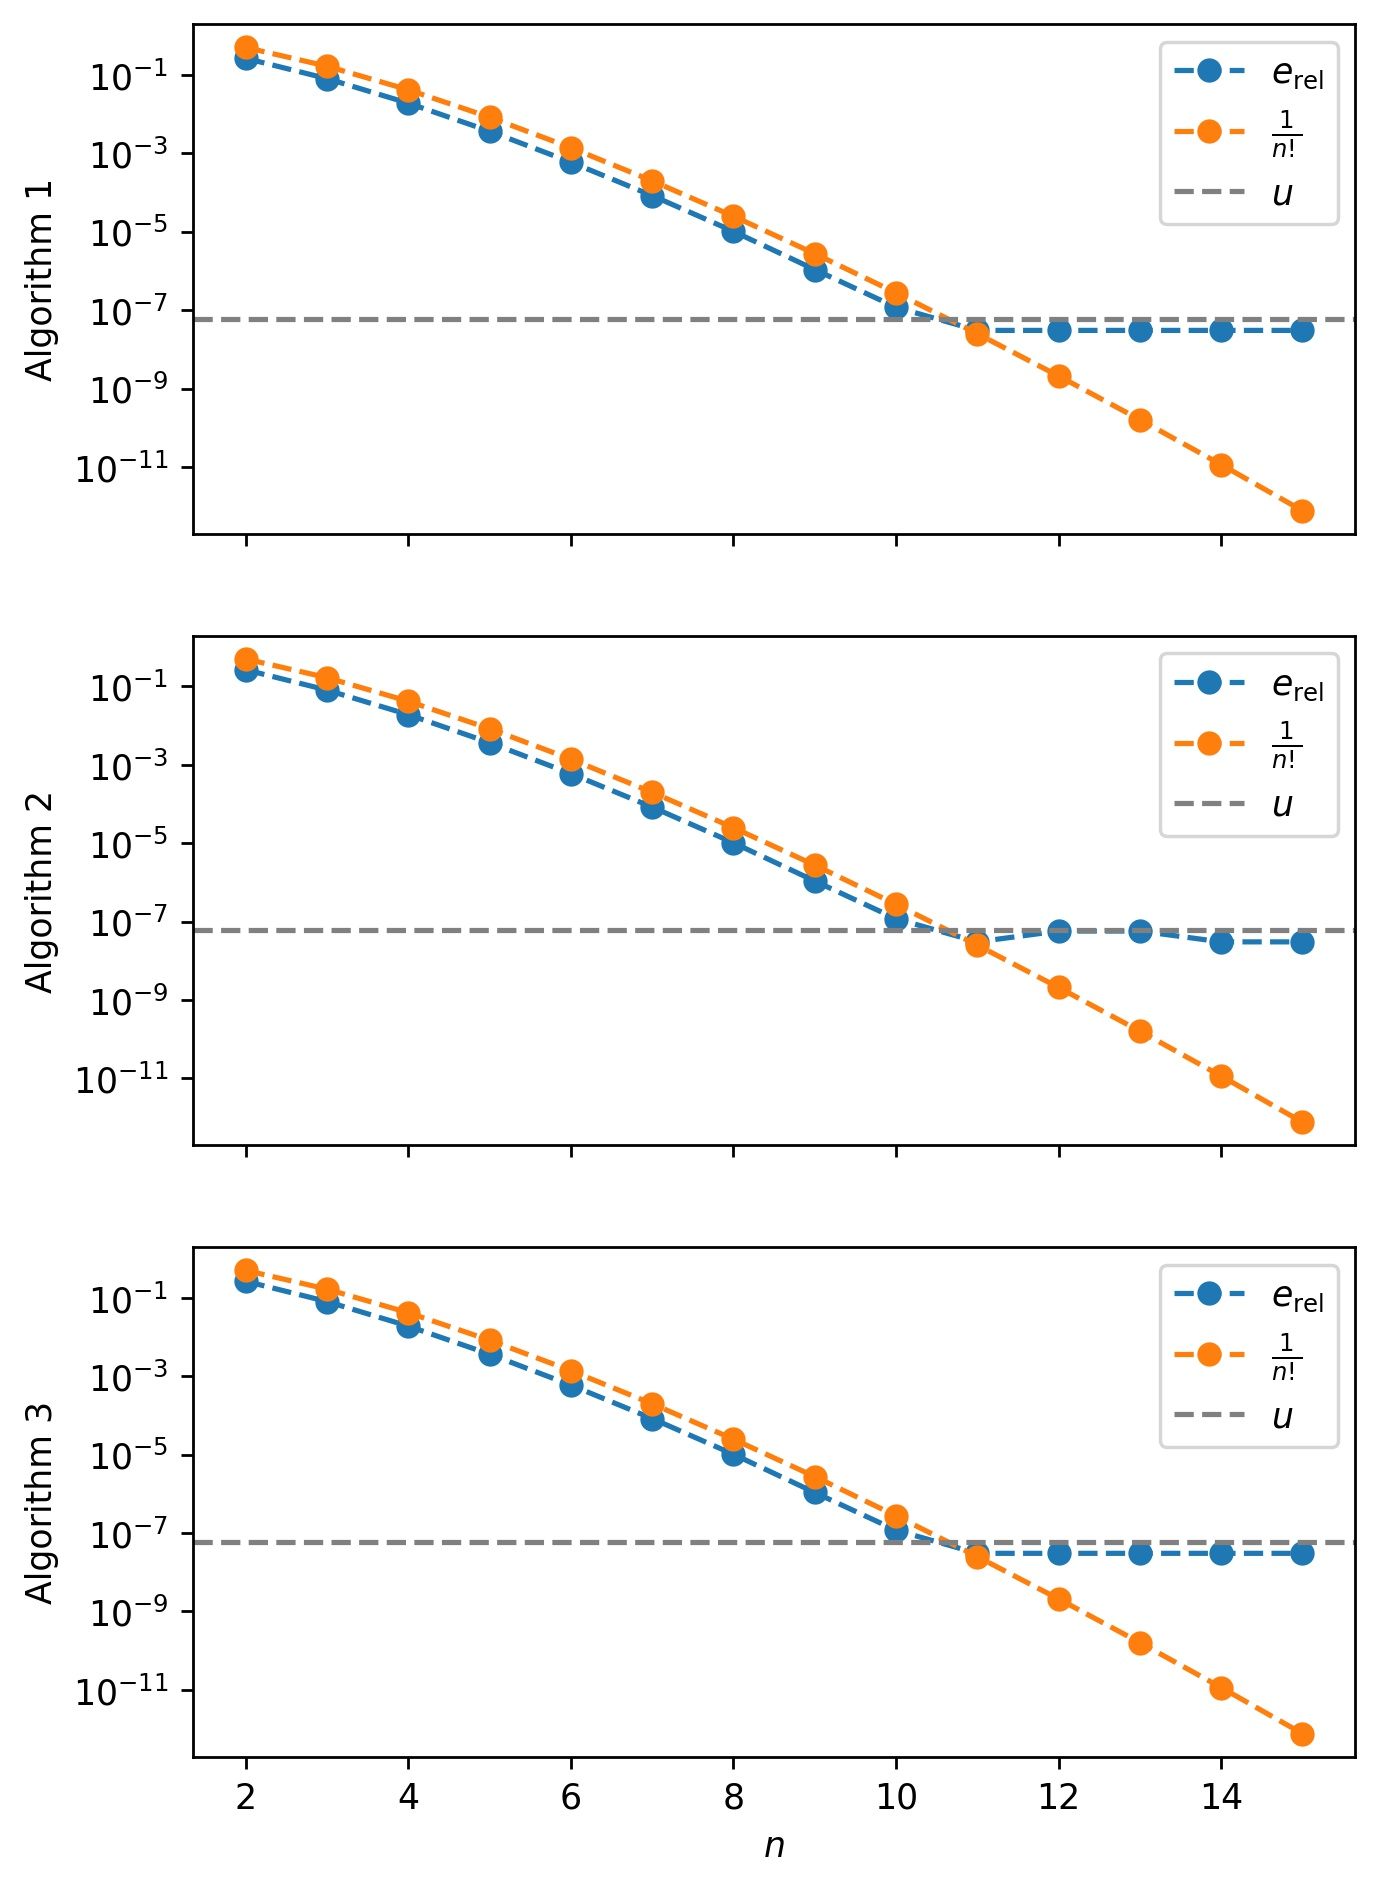
\includegraphics{test1.jpeg}
\caption{Results of test 1. Relative errors of partial Taylor series against upper bounds.}
\label{test1}
\end{figure}

\begin{figure}[H]
\centering
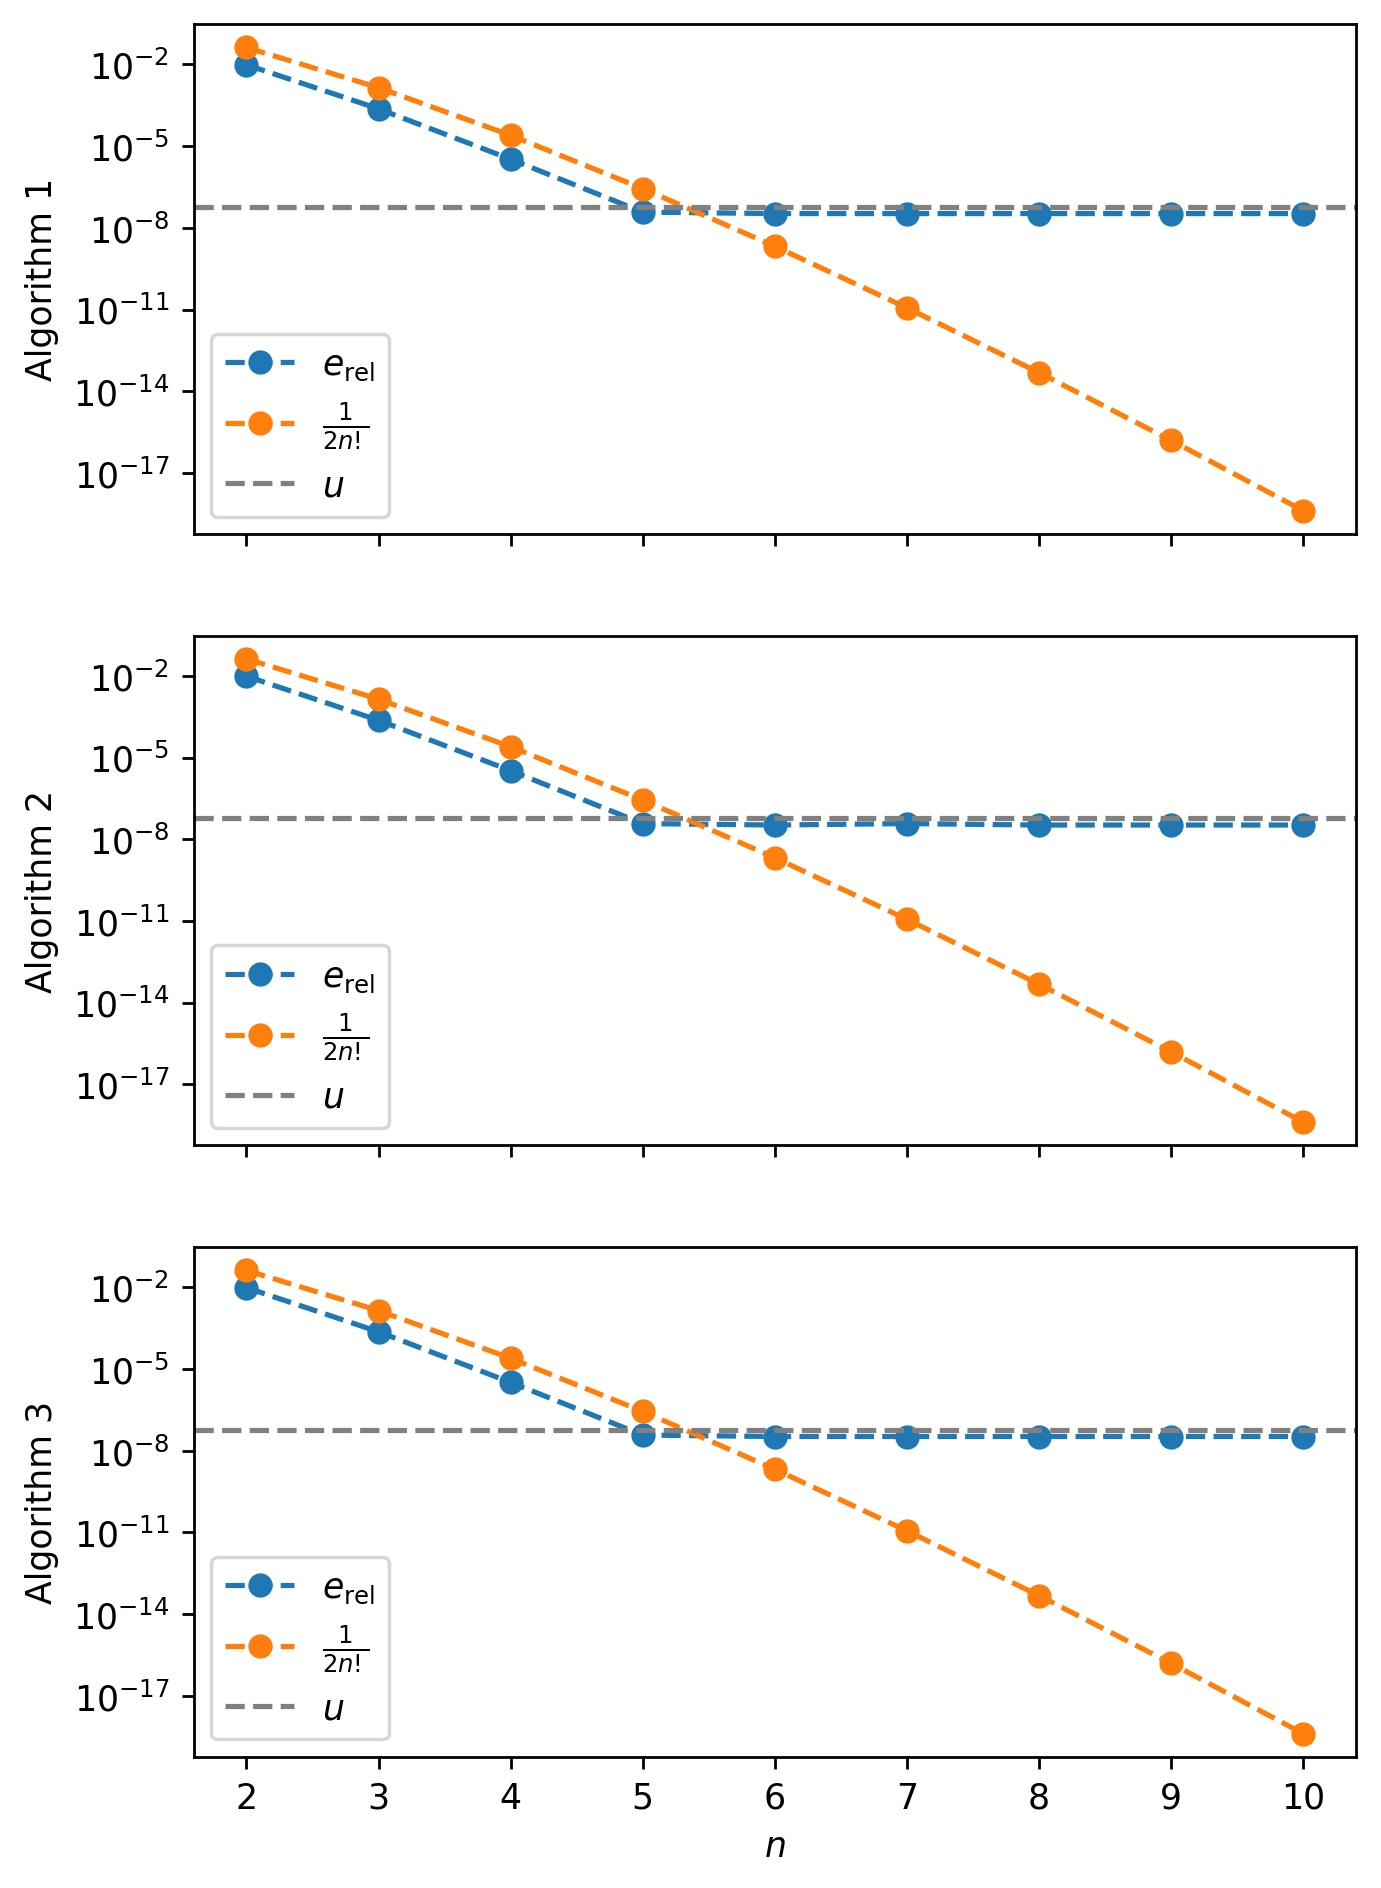
\includegraphics{test2.jpeg}
\caption{Results of test 2. Similar to test 1.}
\label{test2}
\end{figure}

\begin{figure}[H]
\centering
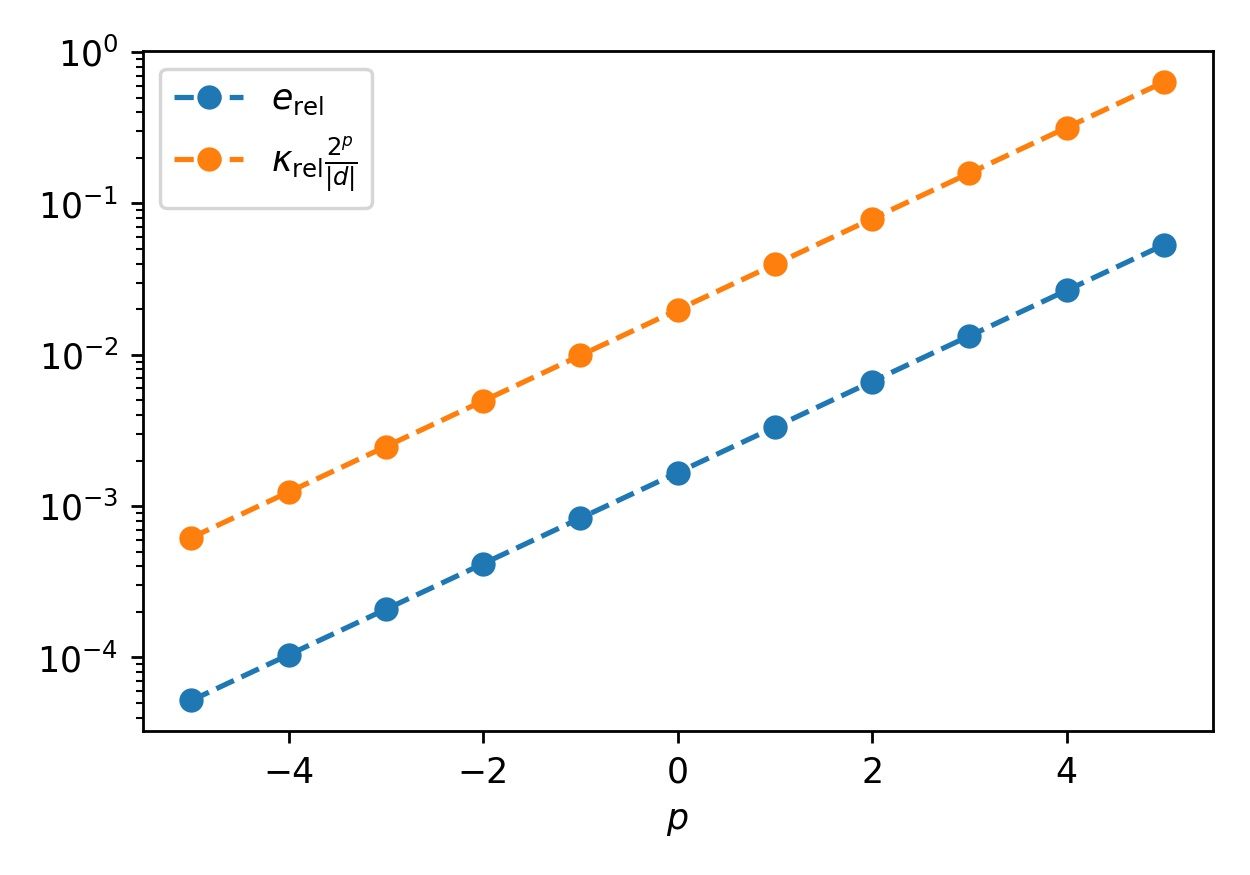
\includegraphics{test3.jpeg}
\caption{Results of test 3. Relative changes in solution against ``scale'' of perturbation.}
\label{test3}
\end{figure}

\begin{figure}[H]
\centering
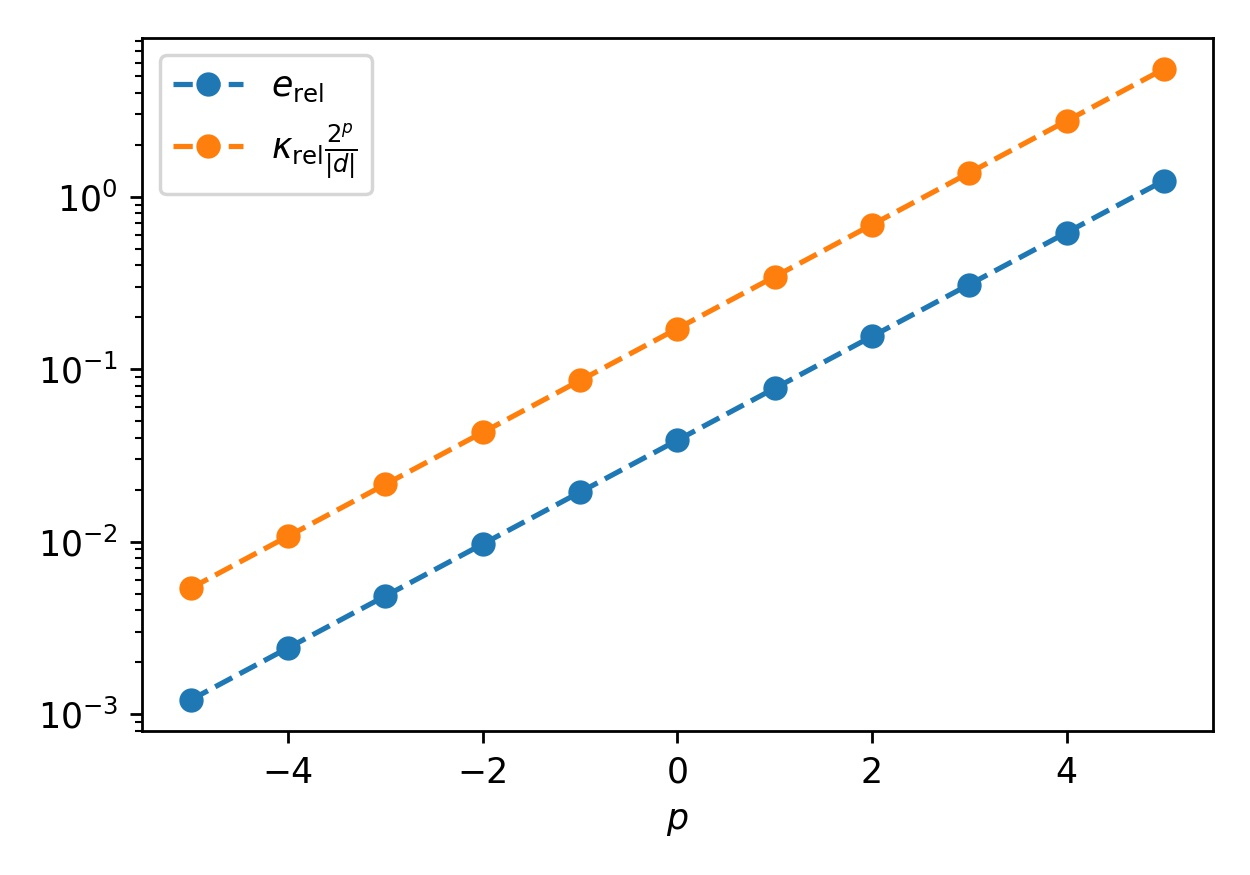
\includegraphics{test4.jpeg}
\caption{Results of test 4. Similar to test 3.}
\label{test4}
\end{figure}

\begin{figure}[H]
\centering
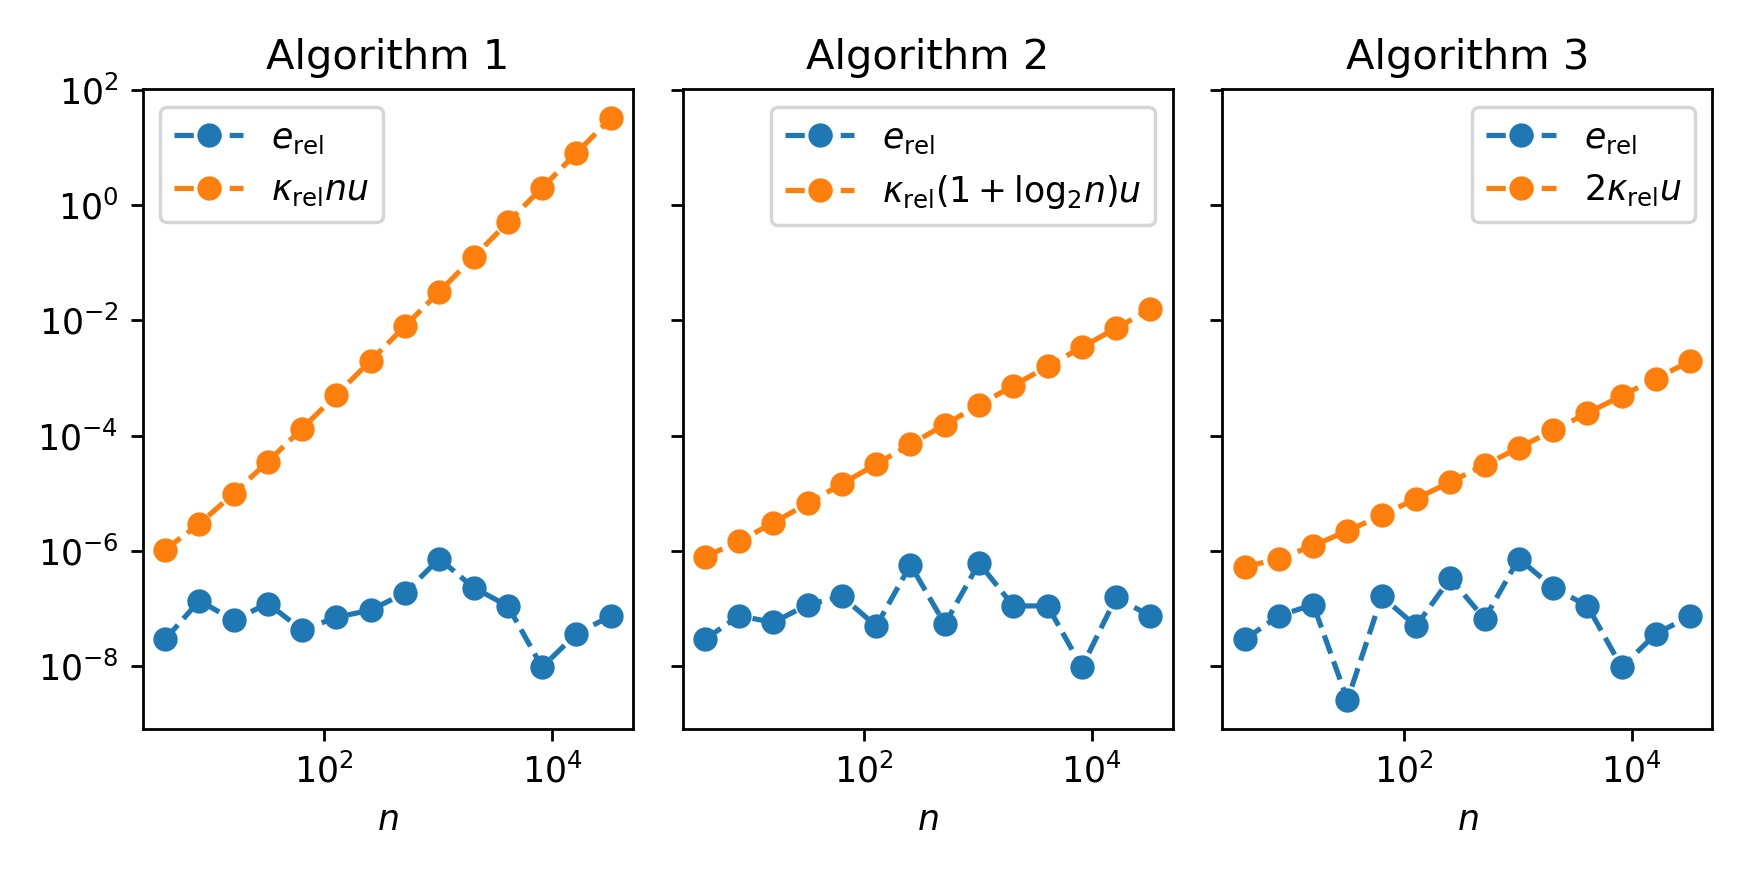
\includegraphics{test5.jpeg}
\caption{Results of test 5. Accumulated rounding error versus upper bounds.}
\label{test5}
\end{figure}

\begin{figure}[H]
\centering
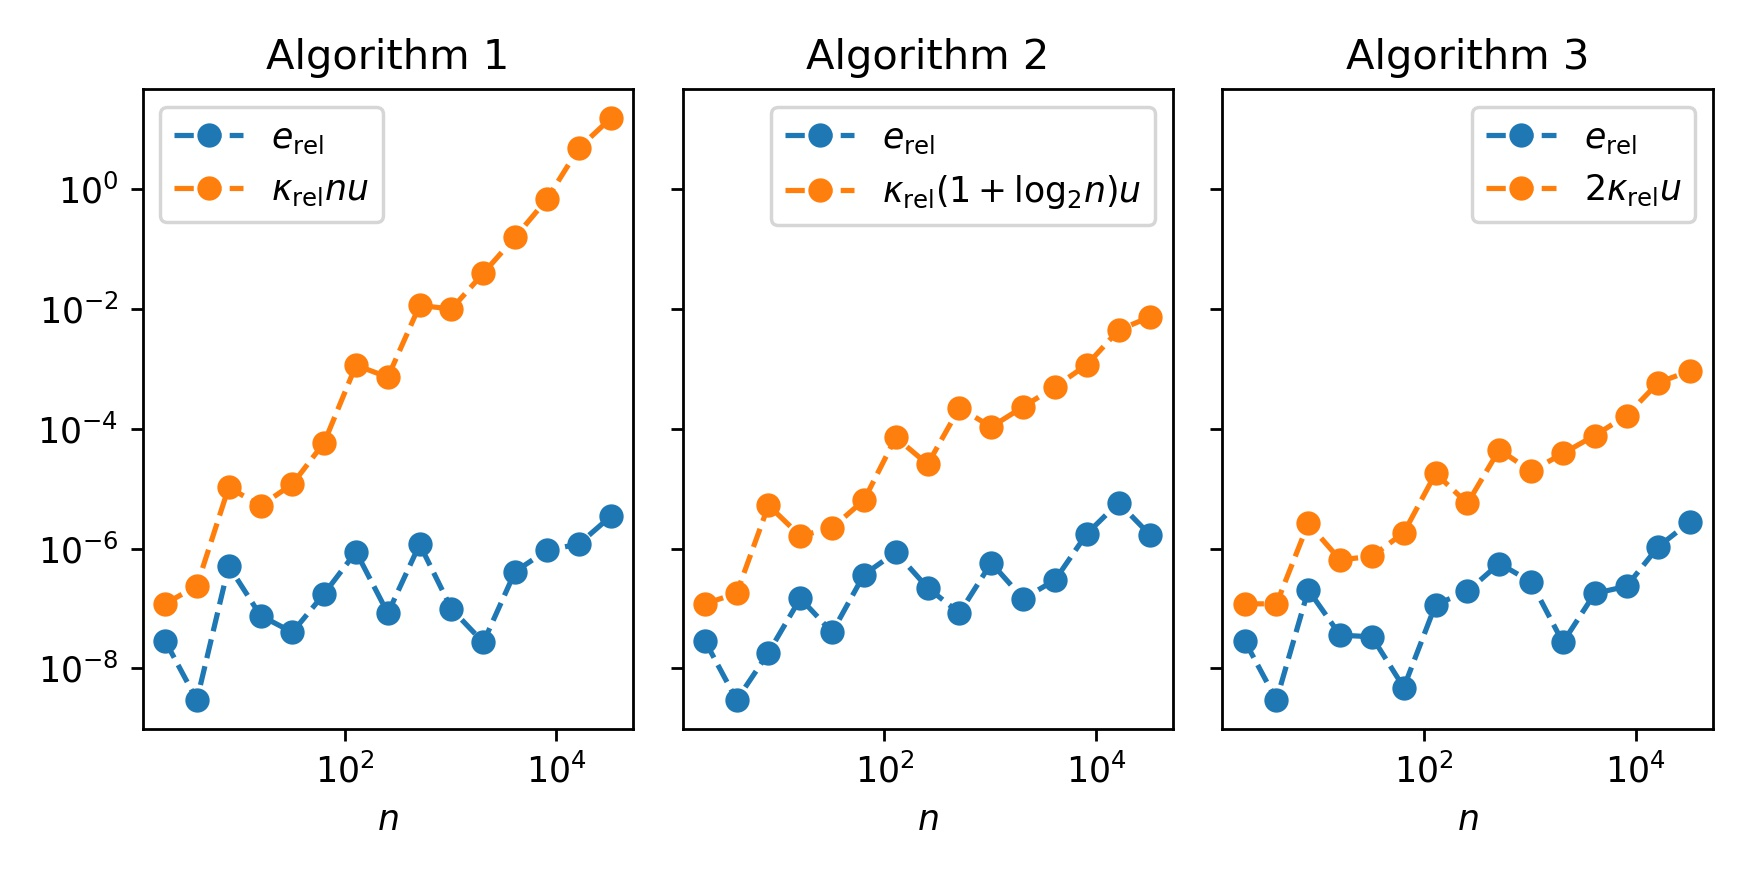
\includegraphics{test6.jpeg}
\caption{Results of test 6. Similar to test 5.}
\label{test6}
\end{figure}

\section{Conclusions}
Our algorithms are accurate. Figures \ref{test1} and \ref{test2} compare the relative error on each term of the sum against the upper bound given by Taylor's remainder theorem. The error consistently falls below the bound until they drop below unit round off $u$, at which point the sum becomes fixed, for new terms are too small to change it. In actuality, we have the more accurate bound $\mathrm{err}_{\text{rel}} \leq \max\cbr{C\frac{1}{n!},u}$.

Summation as a computational problem enjoys well conditioning. Bounded changes in the summands result in bounded changes in the solution. The mathematics of section 3 shows this, and the results of tests 3 and 4 agree with this. In test 3, we added random, but bounded, noise to the summands $1,2,\dots,100$ and showed that the solution $5050$ does not change (in relative value) by more than $\kappa_r \frac{M}{\norm{\mathbf{d}}}$. This is depicted in figure \ref{test3}, which plots the change in the solution against the ``scale'' of perturbation, given by $p$ in $M = 2^p$. For small $(p = -5)$ and large $(p = 5)$ perturbations alike, the upper bound we have proves to be reliable. Figure \ref{test4} argues the same conclusion, except with the summands $2^{-5},2^{-4},\dots,2^5$.

The three algorithms we propose are all backwards stable. We have shown the mathematics in section 3, yet tests 5 and 6 only verify that our algorithms are weakly stable. Figures \ref{test5} and \ref{test6} demonstrate that the upper bounds $\kappa_{\text{rel}}$ are accurate for each of the three algorithms. In fact, they are quite loose, for the relative error grows far slower than the bounds even for large $n$. This implies that the computed solution is always near the exact solution. That the computed solution solves a ``nearby'' problem has only been shown mathematically.

\section{Program Files}
There are three computational units, all written in \texttt{C++}. These are entitled \texttt{main.cpp}, \texttt{tests.cpp}, and \texttt{functions.cpp}. Once in the \texttt{Code} directory, each \texttt{cpp} file may be compiled using \texttt{gcc} with the terminal commands
\begin{verbatim}
g++ main.cpp -c
g++ tests.cpp -c
g++ functions.cpp -c
\end{verbatim}
Then, the resulting object files can be linked using the command
\begin{verbatim}
g++ main.o tests.o functions.o -o program
\end{verbatim}
which produces an executable file named \texttt{program}. The executable can be ran with the line
\begin{verbatim}
program.exe
\end{verbatim}
The code to produce the graphics is written in \texttt{Python} and contained in the file \texttt{plot.py}. The current environment needs the libraries \texttt{numpy} and \texttt{matplotlib} to run the code
\begin{verbatim}
python plot.py
\end{verbatim}

\newpage 
\begin{thebibliography}{9}
\bibitem{lec2}
Gallivan, K. A. \textit{Set 2: Representation, Conditioning and Error}, Lecture Notes. Foundations of Computational Math 1, Florida State University.

\bibitem{lec3}
Gallivan, K. A. \textit{Set 3: Finite Precision Arithmetic and Numerical
Stability}, Lecture Notes. Foundations of Computational Math 1, Florida State University.

\bibitem{lec4}
Gallivan, K. A. \textit{Set 4: Numerical Stability Examples}, Lecture Notes. Foundations of Computational Math 1, Florida State University.

\bibitem{mpl}
J. D. Hunter, ``Matplotlib: A 2D Graphics Environment", Computing in Science \& Engineering, vol. 9, no. 3, pp. 90-95, 2007.

\bibitem{kincaid}
Kincaid, D. \& Cheney, W. (2002) \textit{Numerical Analysis: Mathematics of Scientific Computing}. Brooks/Cole.

\bibitem{quateroni}
Quarteroni, A., Sacco, R., \& Saleri, R. (2000). \textit{Numerical Mathematics}. Springer.
\end{thebibliography}

\end{document}